\documentclass{standalone}

\usepackage{amsmath}
\usepackage{tikz}

\DeclareMathOperator*{\argmin}{argmin}

\usetikzlibrary{shapes, arrows.meta, positioning, backgrounds}

\tikzstyle{block} = [rectangle, minimum width=1cm, minimum height=1cm, text centered, draw=black, fill=white]
\tikzstyle{circ} = [circle, minimum width=.5cm, minimum height=.5cm, text centered, draw=black, fill=white]
\tikzstyle{arrow} = [->,>=stealth]
\tikzstyle{line} = [-,>=stealth]

\begin{document}
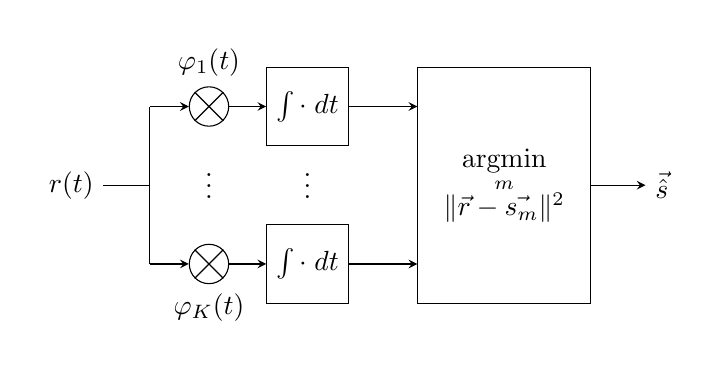
\begin{tikzpicture}[node distance=3cm, background rectangle/.style={fill=white}, show background rectangle]

    \node (rt) at (0, 0) {$r(t)$};
    \node [label=above:$\varphi_1 (t)$] (phi1) [circ] at (1.75, 1) {};
    \node [label=below:$\varphi_K (t)$] (phiK) [circ] at (1.75, -1) {};
    \node (phiN) at (1.75, 0.1) {\vdots};
    \node (int1) [block] at (3, 1) {$\int \cdot \; dt$};
    \node (int2) [block] at (3, -1) {$\int \cdot \; dt$};
    \node (intN) at (3, 0.1) {\vdots};
    \node (argmin) [block, minimum height=3cm] at (5.5, 0) {\begin{tabular}{c} $\argmin_m\limits$ \\ $\| \vec{r} - \vec{s_m} \|^2$ \end{tabular}};
    \node (s) at (7.5, 0) {$\vec{\hat{s}}$};

    \draw [line] (phi1.south east) -- (phi1.north west) (phi1.south west) -- (phi1.north east);
    \draw [line] (phiK.south east) -- (phiK.north west) (phiK.south west) -- (phiK.north east);

    \draw [line] (rt) -- (1, 0);
    \draw [line] (1, 0) -- (1, 1);
    \draw [line] (1, 0) -- (1, -1);
    \draw [arrow] (1, 1) -- (phi1);
    \draw [arrow] (1, -1) -- (phiK);
    \draw [arrow] (phi1) -- (int1);
    \draw [arrow] (phiK) -- (int2);
    \draw [arrow] (int1) -- (int1 -| argmin.west);
    \draw [arrow] (int2) -- (int2 -| argmin.west);
    \draw [arrow] (argmin) -- (s);

\end{tikzpicture}
\end{document}